\documentclass[12pt,german]{article}
\usepackage{listings}
%\usepackage[utf8]{inputenc}
\usepackage{inputenc}
\usepackage{graphicx}
\usepackage{float}
\usepackage{array}
\usepackage{pdfpages}
\usepackage{lscape}

\lstset{
extendedchars=\true,
language=JAVA,
numbers=left, 
numberstyle=\footnotesize, 
%inputencoding=utf8,
%basicstyle=\ttfamily,
%basicstyle=\ttfamily\fontsize{8}{8},
%commentstyle=\ttfamily\fontsize{8}{8},
basicstyle=\tiny;
columns=fullflexible,
%xleftmargin=5pt,
frame=single,
breaklines=true,
postbreak=\mbox{{$\hookrightarrow$}\space},
}
\renewcommand{\thesubsubsection}{\alph{subsubsection} )}
%\renewcommand{\thesubsubsection}{\thesubsection.\alph{subsubsection} )}

\setcounter{section}{3}

\begin{document}

\title{Übungsaufgaben IV, SBV1 }
\author{Lukas Fiel, Lisa Panholzer}
\maketitle


\newpage
\section{Übungsaufgaben IV}
\subsection{Region Growing}

\subsubsection{Manuelles Image Growing}
\label{subsec:manualRegionGrowing}
Der Algorithmus zu dieser Übung wurde aus der Vorlesung übernommen. Es waren lediglisch N4 und N8 Nachbarpixelregionen zu unterscheiden. Diese wurden einfach durch Variable der Funktion mitgegeben und in einer \textit{if} Abfrage abgefragt. \\
Figure \ref{tab:N4pattern} und Figure \ref{tab:N8pattern} vergleichen die zu unersuchenden Nachbarschaftspixel.

\textit{Regionsvergleich}

\begin{table}[H]
  \centering
  \begin{tabular}{| c | c  c  c |}
    \hline
    x/y & -1 & 0 & 1 \\
    \hline
    -1  & 0 & x & 0 \\
    0   & x & 0 & x \\
    1   & 0 & x & 0 \\
    \hline
  \end{tabular}
  \caption{N4 Region}
  \label{tab:N4pattern}

  \hspace{1cm}

  \begin{tabular}{| c | c  c  c |}
    \hline
    x/y & -1 & 0 & 1 \\
    \hline
    -1  & x & x & x \\
    0   & x & 0 & x \\
    1   & x & x & x \\
  \hline
  \end{tabular}
  \caption{N8 Region}
  \label{tab:N8pattern}
\end{table}


\begin{landscape}
\lstinputlisting[frame=single,language=JAVA,breaklines=true,caption = RegionGrowing-Algorithmus.]{../../RegionGrowing_.java}
\end{landscape}


\subsubsection{Image Growing mit Labeling}
Für die Implmentierung wurde der Code aus Aufgabe \ref{subsec:manualRegionGrowing} kopiert und erweitert. Muss das gesamte Bild untersucht werden um alle Objekte zu finden. Wird ein passendes Pixel gefunden, wird der Region-Growing Algorithmus herangezogen. Mittels der Fordergrundfarbe werden die Objekte eingeteilt und unterschieden.

\begin{landscape}
\lstinputlisting[frame=single,language=JAVA,breaklines=true,caption = RegionGrowing-Algorithmus]{../../AutoRegionGrowing_.java}
\end{landscape}


\subsection{Optimaler Threshold}
Der zum Start benötigte initiale Threshold wird anhand eines User Inputs definiert. Wird kein Input angegeben wird als Default-Wert 127 gesetzt (255/2), somit startet die Berechnung mittig vom Histogramm.\\
Um mit der Berechnung des optimalen Threshold starten zu können wurden zwei Konstanten FG\_VAL und BG\_VAL definiert, die die jeweils kleinste und höchste Intensität enthalten.  Bei jeder Iteration wird geprüft, ob der aktuelle Wert des Eingangsbildes über oder unter dem Threshold Wert. Liegt der Wert darunter, wird dieser in der sumThresh01 Variable aufsummiert und der Counter erhöht. Ist der Wert darüber, passiert dasselbe nur mit anderen Variablen.\\
Die aufsummierten Werte der zwei Bereiche werden nun benötigt um nach durlaufen des Eingangsbildes den Durchschnitt zu berechnen. Der vorübergehende Threshold wird aus den beiden meanThresh01, meanThresh02 berechnet. Nun wird geprüft, ob das Delta das sich zwischen dem vorübergehenden und initialen Threshold ergibt, über der definierten Konvergenz (DELTA\_VAL), in diesem Fall 0.01, liegt. Wenn ja, wird ein erneuter Schleifendurchlauf gestartet. Wenn die Werte gleich sind, wird die Schleife abgebrochen und das berechnete Ausgangsbild ausgegeben.


\begin{table}[H]
  \centering
  \begin{tabular}{| c | c | c | c | }
    \hline
   initialer \\Threshold Wert & Eingangsbild & Optimal Threshold & Threshold Bild \\
    \hline
     60 & 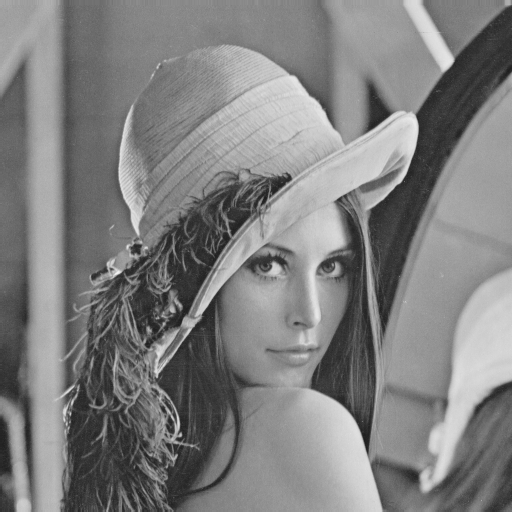
\includegraphics[width=5cm]{../Bilddaten/3_lena.png} &  117.81496778947292; & 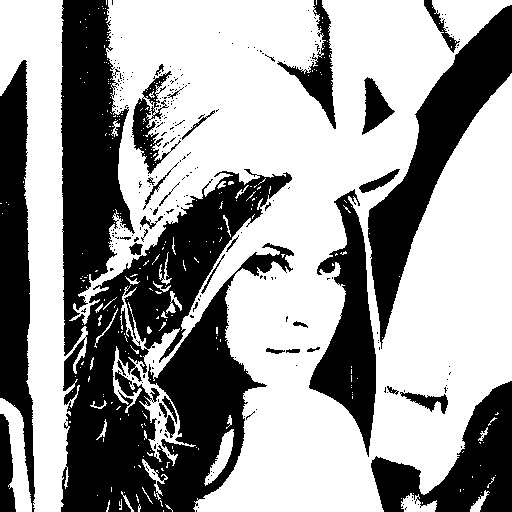
\includegraphics[width=5cm]{../Bilddaten/threshold_image-01.png}\\
\hline
 127 & 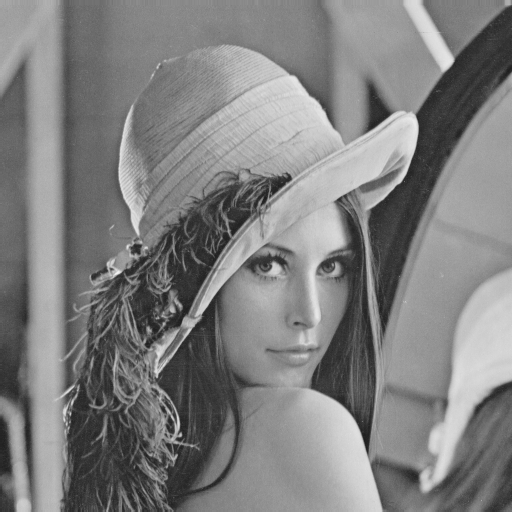
\includegraphics[width=5cm]{../Bilddaten/3_lena.png} &    120.52898065546574  & 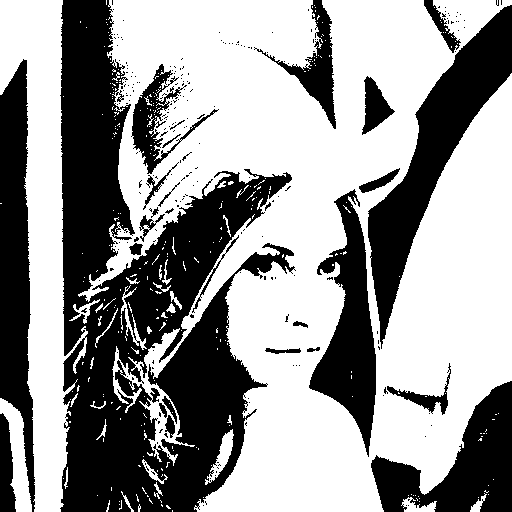
\includegraphics[width=5cm]{../Bilddaten/threshold_image-02.png} \\
\hline
     
  \end{tabular}
  \caption{Optimal Threshold Testbilder}
\end{table}


\lstinputlisting[frame=single,language=JAVA,breaklines=true,caption = Optimal Threshold Algorithmus]{../../OptimalThreshold_.java}


\subsubsection{Adaptiver optimar Threshold}

Um den Filter des Optimal Threshold auch bei Bildern gut einsetzen zu können, die unterschiedliche Intensitätsverteilung pro Sektor haben, wurde der Adaptive Threshold-Filter implementiert.

Dieser verwendet die Funktionalität des Optimal Threshold wendet diese jedoch auf Sektoren mit einer Größe von 100x100 Pixel an. Die Sektoren werden aus dem Bild herausgeschnitten, der Optimal Threshold berechnet und zwischengespeichert. Abschließend werden Sie zu einem Bild zusammen gesetzt und ausgegeben.

\begin{table}[H]
  \centering
  \begin{tabular}{| c | c | c | c | }
    \hline
   initialer \\Threshold Wert & Eingangsbild &  Threshold Bild \\
    \hline
     60 & 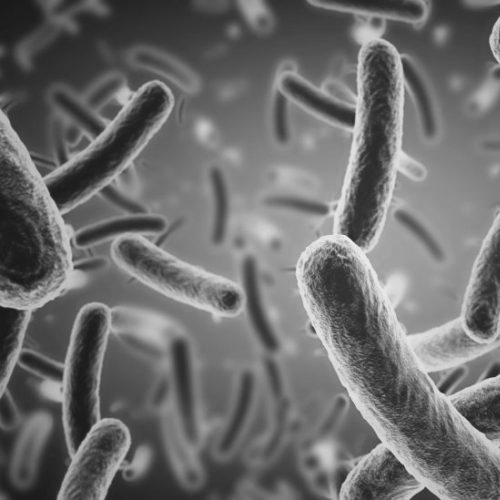
\includegraphics[width=5cm]{../Bilddaten/bacteria.png} &   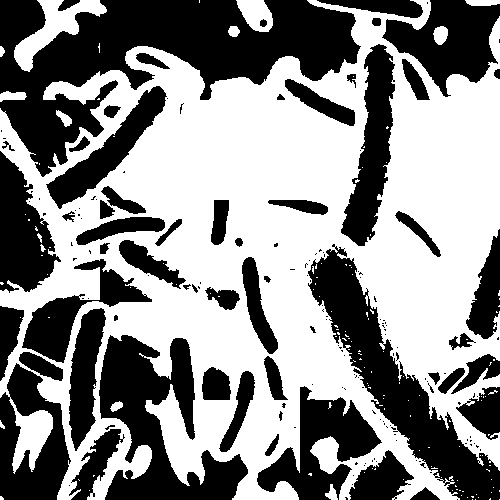
\includegraphics[width=5cm]{../Bilddaten/bacteria-01.png}\\
\hline
 127 & 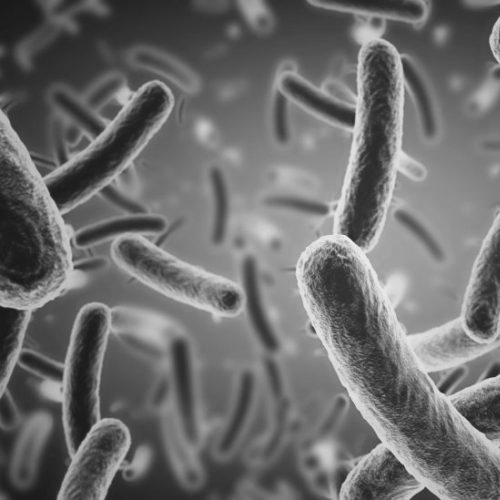
\includegraphics[width=5cm]{../Bilddaten/bacteria.png} &     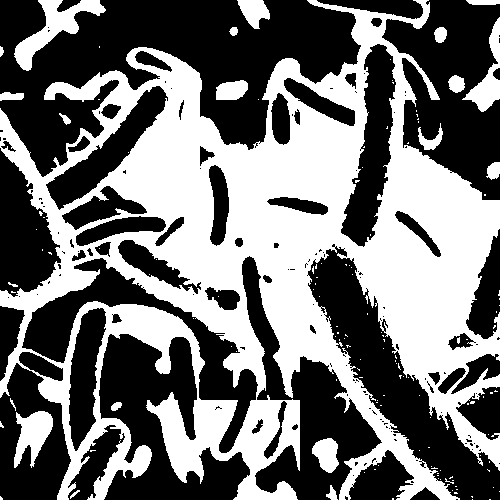
\includegraphics[width=5cm]{../Bilddaten/bacteria-02.png} \\
\hline
     
  \end{tabular}
  \caption{Adaptive Threshold Testbilder}
\end{table}

\lstinputlisting[frame=single,language=JAVA,breaklines=true,caption = Adaptive Threshold Algorithmus]{../../AdaptiveThreshold_.java}


\end{document}
